%%%%%%%%%%%%%%%%%%%%%%%%%%%%%%%%%%%%%%%%%
% Freeman Curriculum Vitae
% XeLaTeX Template
% Version 3.0 (September 3, 2021)
%
% This template originates from:
% https://www.LaTeXTemplates.com
%
% Authors:
% Vel (vel@LaTeXTemplates.com)
% Alessandro Plasmati
%
% License:
% CC BY-NC-SA 4.0 (https://creativecommons.org/licenses/by-nc-sa/4.0/)
%
%!TEX program = xelatex
% NOTE: this template must be compiled with XeLaTeX rather than PDFLaTeX
% due to the custom fonts used. The line above should ensure this happens
% automatically, but if it doesn't, your LaTeX editor should have a simple toggle
% to switch to using XeLaTeX.
% 
%%%%%%%%%%%%%%%%%%%%%%%%%%%%%%%%%%%%%%%%%

%----------------------------------------------------------------------------------------
%	PACKAGES AND OTHER DOCUMENT CONFIGURATIONS
%----------------------------------------------------------------------------------------

\documentclass[
	10pt, % Default font size, can be between 8pt and 12pt
]{FreemanCV}

\columnratio{0.55, 0.45} % Widths of the two columns, specified here as a ratio summing to 1 to correspond to percentages; adjust as needed for your content 

% Headers and footers can be added with the following commands: \lhead{}, \rhead{}, \lfoot{} and \rfoot{}
% Example right footer:
%\rfoot{\textcolor{headings}{\sffamily Last update: \today. Typeset with Xe\LaTeX}}

%----------------------------------------------------------------------------------------

\begin{document}

\begin{paracol}{2} % Begin two-column mode

%----------------------------------------------------------------------------------------
%	YOUR NAME AND CURRICULUM VITAE TITLE
%----------------------------------------------------------------------------------------

\parbox[][0.11\textheight][c]{\linewidth}{ % Box to hold your name and CV title; change the fixed height as needed to match the colored box to the right
	\centering % Horizontally center text
	
	{\sffamily\Huge Sebastian Peschke} % Your name
	
	\medskip % Vertical whitespace
	
	{\cursivefont\Huge\textcolor{headings}{Curriculum Vitae}}
	
	\vfill % Push content to the top of the box
}


\section{Persönliche Daten}
\begin{supertabular}{r l} % Start a table with two columns, the table will ensure everything is aligned
	%------------------------------------------------
	%\tableentry{Position}{Professor}{}

	\tableentry{Name}{\textbf{Sebastian Peschke}}{spaceafter}
	\tableentry{Geboren am}{30.07.2000}{}
	\tableentry{Anschrift}{Jahnstraße 6a}{}
	\tableentry{}{95030 Hof an der Saale}{}
	\tableentry{E-Mail}{sebastian.peschke@hof-university.de}{}
	\tableentry{GitHub}{https://github.com/ItsMagick}{}
	\tableentry{TryHackMe}{https://tryhackme.com/p/ItsMagick}{}
	\tableentry{Mobil}{+49 157 34 555 224}{spaceafter}

	\\ % Additional vertical whitespace between the references
	%------------------------------------------------


\end{supertabular}


%----------------------------------------------------------------------------------------
%	MAJOR RESEARCH PROJECT
%----------------------------------------------------------------------------------------


%{\raggedright\textbf{``Observation of Einstein-Podolsky-Rosen Entanglement on Supraquantum Structures by Induction Through Nonlinear Transuranic Crystal of Extremely Long Wavelength Pulse from Mode-Locked Source Array"}\par}

%\medskip % Vertical whitespace
%
%My research examined the use of ELW pulses from a mode-locked source array inducted through transuranic crystals to observe entanglement on supraquantum structures. Theoretical advancements included prediction of quantum resonance phenomena including the possibility of resonance cascades. I was motivated to conduct this doctoral research due to my passion for teleportation of matter and I believe I have laid the foundation for further experimental validation and development of practical outcomes.
%
%\medskip % Extra vertical whitespace before the next section

%----------------------------------------------------------------------------------------
%	WORK EXPERIENCE
%----------------------------------------------------------------------------------------

\section{Berufliche Laufbahn}

% Each job is added with a \jobentry command. Below is an empty one to use as a template:

%\jobentry
%	{} % Duration
%	{} % FT/PT (full time or part time)
%	{} % Employer
%	{} % Job title
%	{} % Description

% All 5 parameters must be supplied but any can be empty if you don't need them

%------------------------------------------------

\jobentry
{15.03.23 - 07.07.23} % Duration
{TZ} % FT/PT (full time or part time)
{Institut für Informationssysteme, \\ Forschungsgruppe System and Network Security \newline} % Employer
{Studentische Hilfskraft} % Job title
{Als Studentische Hilfskraft unterstütze ich die Forschungsgruppe \newline System and Network Security im Thema
	Rowhammer} % Description

%------------------------------------------------


%----------------------- -----------------------------------------------------------------
%	REFERENCES
%----------------------------------------------------------------------------------------


%\textit{References available on request} % Uncomment if you'd rather not include references and remove the section below

%------------------------------------------------

% This section is laid out using a table. A \tableentry command adds lines with the following parameters:

%\tableentry{Heading}{Content}{spaceafter}
% All 3 parameters must be supplied but any can be empty if you don't need them
% A "spaceafter" value in the third parameter will add some vertical space -- this is to be used between headings, leave it empty for no extra space

%------------------------------------------------




\medskip % Extra vertical whitespace before the next section

%----------------------------------------------------------------------------------------


%----------------------------------------------------------------------------------------
%	COLORED CONTACT DETAILS BOX
%----------------------------------------------------------------------------------------
%
%\parbox[top][0.11\textheight][c]{\linewidth}{ % Box to hold the colored box; change the fixed height as needed to match the box to the left
%	\colorbox{shade}{ % Create colored box and specify background color
%		\begin{supertabular}{@{\hspace{3pt}} p{0.05\linewidth} | p{0.775\linewidth}} % Start a table with two columns, the table will ensure everything is aligned
%			\raisebox{-1pt}{\faHome} & P.O. Box 3985, Black Mesa Drive, NM 87545 \\ % Address
%			\raisebox{-1pt}{\faPhone} & +1 (800) 786-1410 \\ % Phone number
%			\raisebox{-1pt}{\small\faEnvelope} & \href{mailto:g.freeman@bmrf.us}{g.freeman@bmrf.us} \\ % Email address
%			\raisebox{-1pt}{\small\faDesktop} & \href{https://www.LaTeXTemplates.com}{https://www.LaTeXTemplates.com} \\ % Website
%			%\raisebox{-1pt}{\faGithub} & \href{https://github.com/username}{https://github.com/username} \\ % GitHub profile
%			%\raisebox{-1pt}{\faLinkedinSquare} & \href{https://www.linkedin.com/in/username}{https://www.linkedin.com/in/username} \\ % LinkedIn profile
%			% See fontawesome.pdf in the Fonts folder for all icons you can use
%		\end{supertabular}
%	}
%	\vfill % Push content to the top of the box
%}
%
%----------------------------------------------------------------------------------------
%	EDUCATION
%----------------------------------------------------------------------------------------

\section{Schulische Laufbahn}

% Each qualification entry is added with a \qualificationentry command. Below is an empty one to use as a template:

%\qualificationentry
%	{} % Duration
%	{} % Degree
%	{} % Honors, achievements or distinctions (e.g. first class honors)
%	{} % Department
%	{} % Institution

% All 5 parameters must be supplied but any can be empty if you don't need them

%------------------------------------------------

\begin{supertabular}{r l} % Start a table with two columns, the table will ensure everything is aligned

	%------------------------------------------------

	\qualificationentry
	{Juni 2019} % Duration
	{Abitur} % Degree
	{} % Honors, achievements or distinctions (e.g. first class honors)
	{} % Department
	{Schiller-Gymnasium Hof} % Institution

	%------------------------------------------------

	\qualificationentry
	{Okt 2019 - Sep 2020} % Duration
	{Informatik B.Sc.} % Degree
	{Abgebrochen} % Honors, achievements or distinctions (e.g. first class honors)
	{} % Department
	{HAW Hof} % Institution

	%------------------------------------------------

	\qualificationentry
	{Okt 2020 - Sep 2024} % Duration
	{Mobile Computing B.Sc.} % Degree
	{} % Honors, achievements or distinctions (e.g. first class honors)
	{} % Department
	{HAW Hof} % Institution

	%------------------------------------------------

\end{supertabular}
\section{Kenntnisse}



% This section is laid out using a table. A \tableentry command adds lines with the following parameters:



%\tableentry{Heading}{Content}{spaceafter}

% All 3 parameters must be supplied but any can be empty if you don't need them

% A "spaceafter" value in the third parameter will add some vertical space -- this is to be used between headings, leave it empty for no extra space



%------------------------------------------------



\begin{supertabular}{r l} % Start a table with two columns, the table will ensure everything is aligned



	%------------------------------------------------

	\tableentry{Sehr Gut}{Tschechisch, Deutsch (Muttersprache)}{}

	\tableentry{}{Englisch (C1+),}{spaceafter}



	\tableentry{GUT}{Java, Java Script, Kotlin, Swift,}{}

	\tableentry{}{Linux, Gitlab CI/CD,}{}

	\tableentry{}{Scrum, DevOps}{}

	\tableentry{}{Französisch (B1+)}{spaceafter}



	%------------------------------------------------



	\tableentry{Ausreichend}{Python, C, C++, C\#, Flutter, Bash}{}

	%\tableentry{}{Microsoft Windows}{}

	%\tableentry{}{Computer Hardware \& Support}{spaceafter}



	%------------------------------------------------



	%\tableentry{Expert}{Perl, Unix, \LaTeX}{spaceafter}



	%------------------------------------------------



\end{supertabular}

\switchcolumn % Switch to the second (right) column
%----------------------------------------------------------------------------------------
%	AWARDS
%----------------------------------------------------------------------------------------

%\section{Awards}
%
%% This section is laid out using a table. A \tableentry command adds lines with the following parameters:
%
%%\tableentry{Heading}{Content}{spaceafter}
%% All 3 parameters must be supplied but any can be empty if you don't need them
%% A "spaceafter" value in the third parameter will add some vertical space -- this is to be used between headings, leave it empty for no extra space
%
%%------------------------------------------------
%
%\begin{supertabular}{r l} % Start a table with two columns, the table will ensure everything is aligned
%
%	%------------------------------------------------
%
%	\tableentry{1985}{\textbf{Faculty of Science Masters Scholarship}}{}
%	\tableentry{}{\textit{Massachusetts Institute of Technology}}{spaceafter}
%
%	%------------------------------------------------
%
%	\tableentry{1983}{\textbf{Top Achiever Award -- Physics}}{}
%	\tableentry{}{\textit{The University of Washington}}{spaceafter}
%
%	%------------------------------------------------
%
%\end{supertabular}
%ochschule Für Angewandte \newline Wissenschaften \newline
%----------------------------------------------------------------------------------------
%	COMPUTER SKILLS
%----------------------------------------------------------------------------------------

%TODO: Hier Bewerbungsfoto Einfügen
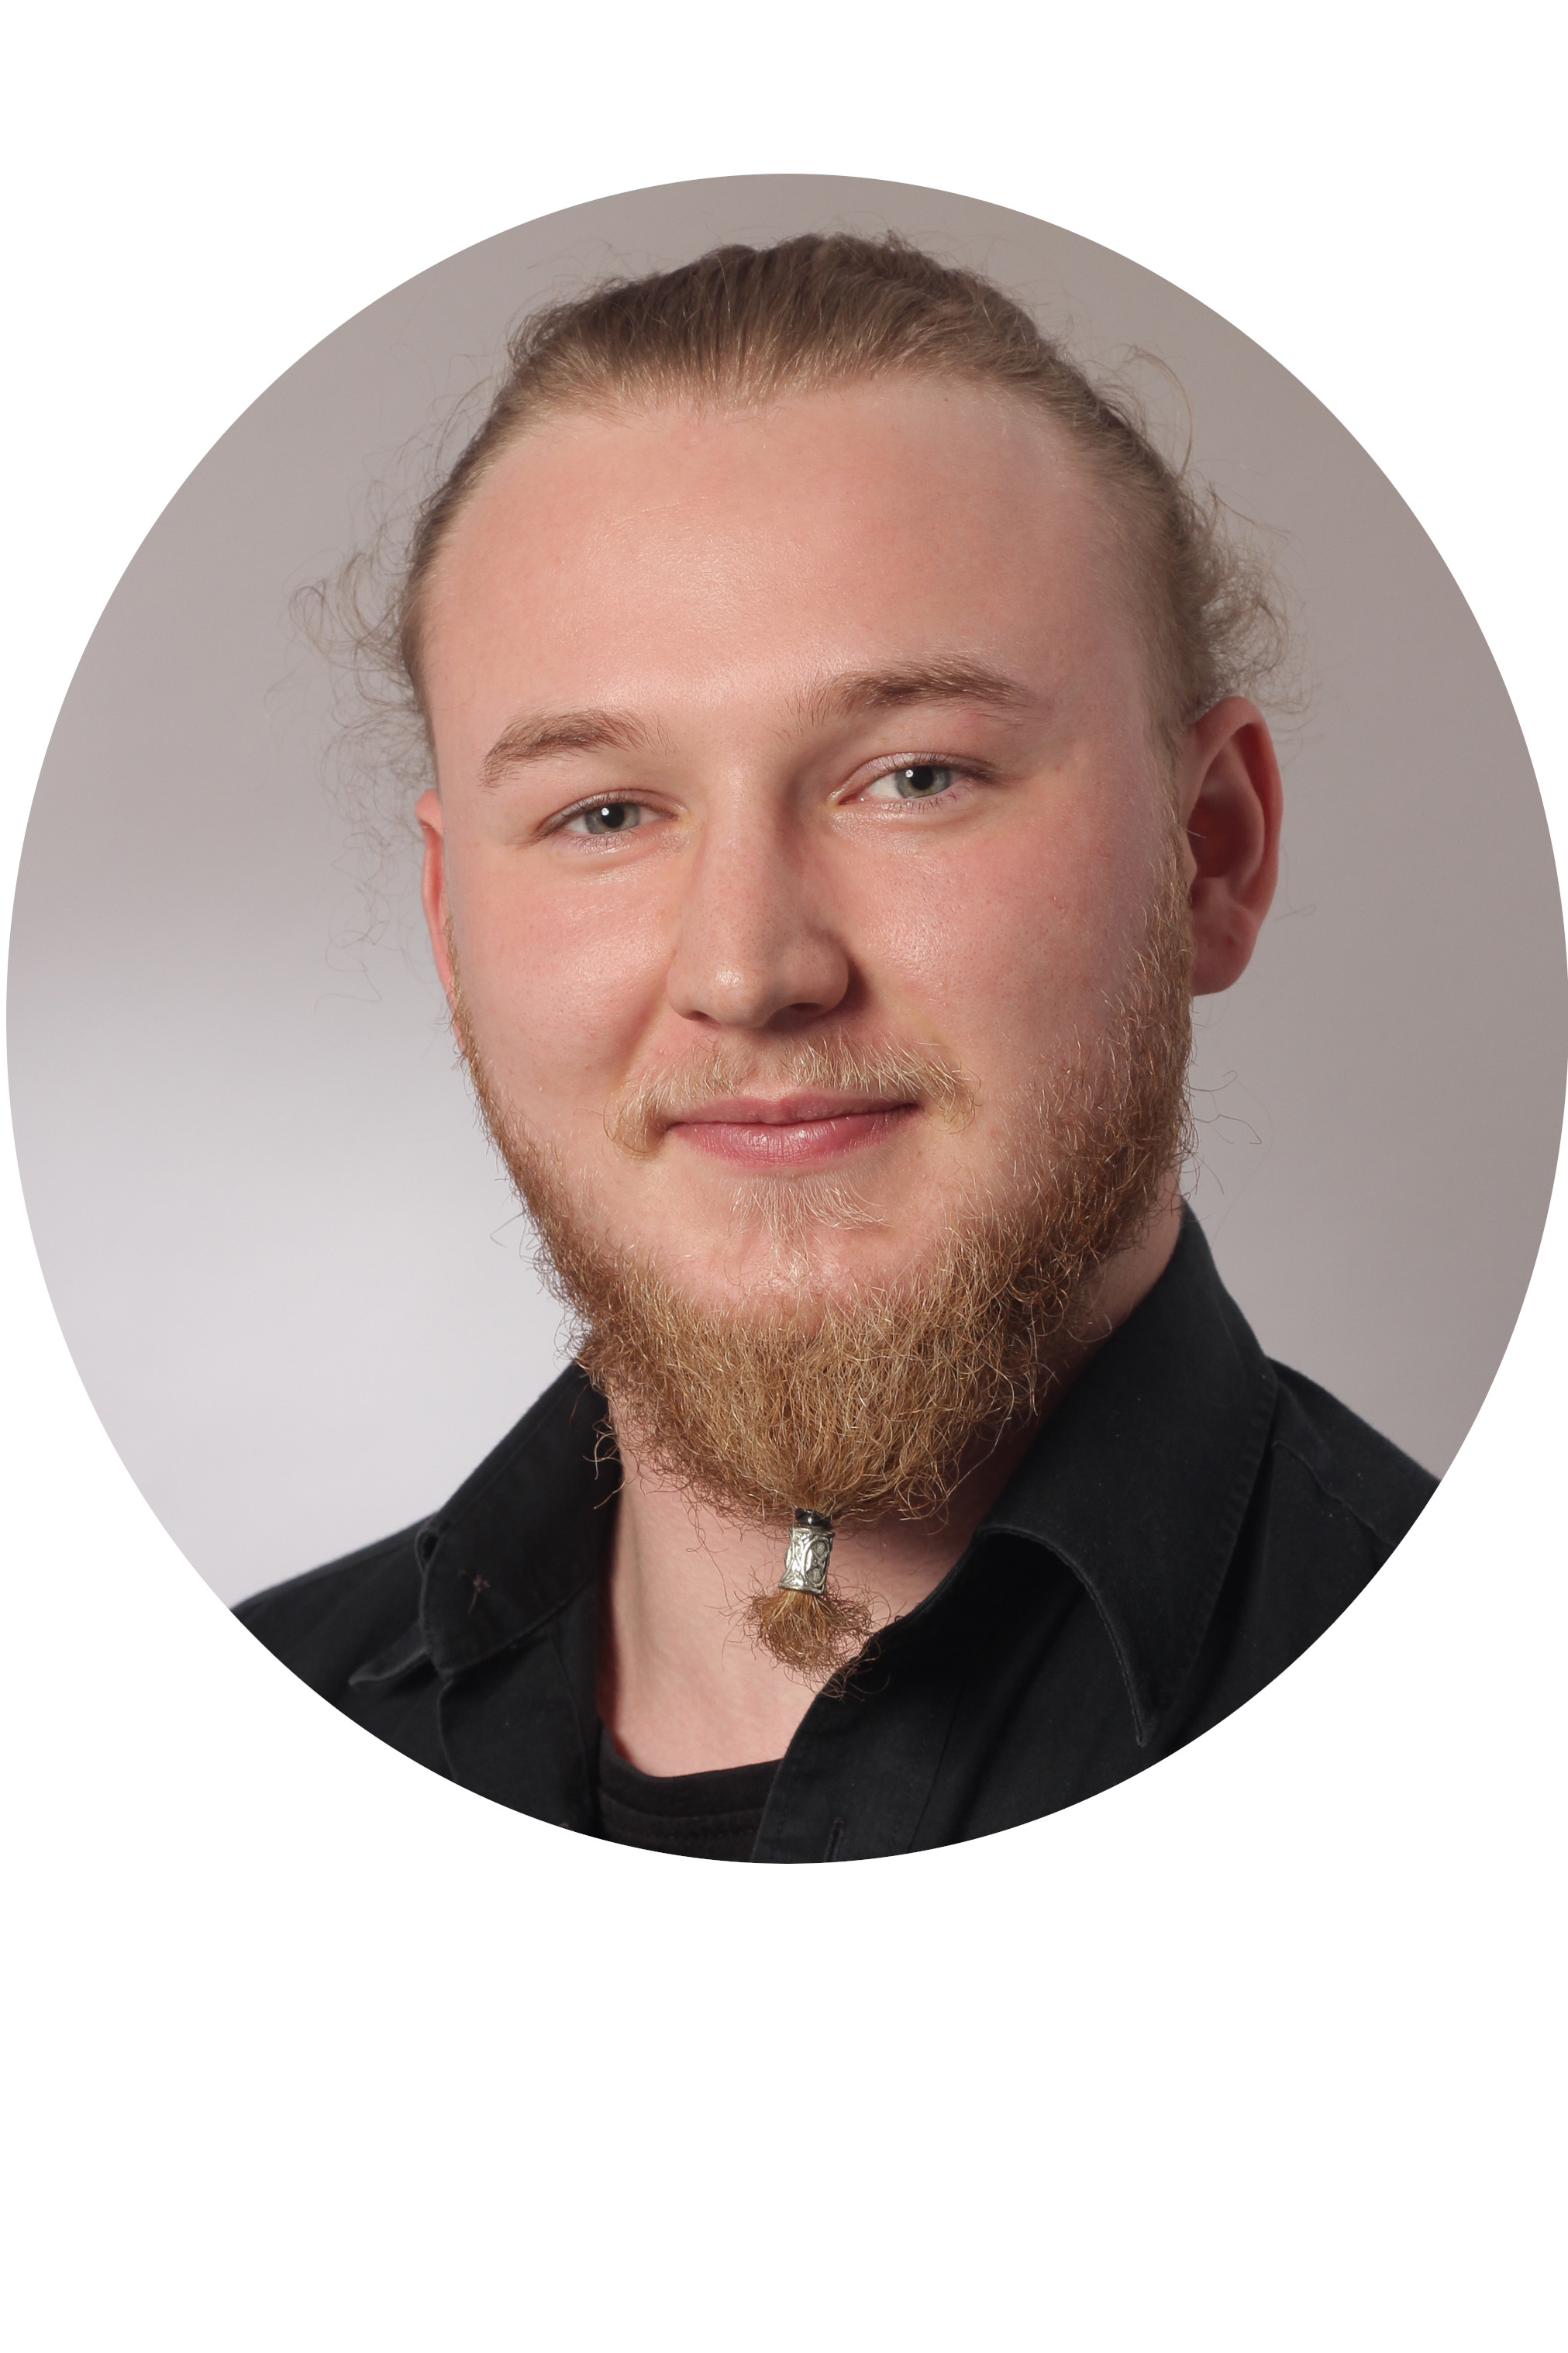
\includegraphics[scale=0.1]{./assets/Peschke Sebastian}
%----------------------------------------------------------------------------------------
%	COMMUNICATION SKILLS
%----------------------------------------------------------------------------------------

%\section{Communication Skills}
%
%% This section is laid out using a table. A \tableentry command adds lines with the following parameters:
%
%%\tableentry{Heading}{Content}{spaceafter}
%% All 3 parameters must be supplied but any can be empty if you don't need them
%% A "spaceafter" value in the third parameter will add some vertical space -- this is to be used between headings, leave it empty for no extra space
%
%%------------------------------------------------
%
%\begin{supertabular}{r l} % Start a table with two columns, the table will ensure everything is aligned
%
%	%------------------------------------------------
%
%	\tableentry{Conferences}{Oral Presentation at the Annual MIT}{}
%	\tableentry{}{Theoretical Physics Conference -- 1987}{spaceafter}
%
%	%------------------------------------------------
%
%	\tableentry{Posters}{Poster at the Meeting of the American}{}
%	\tableentry{}{Physical Society -- 1985}{spaceafter}
%
%	%------------------------------------------------
%
%\end{supertabular}
%
%----------------------------------------------------------------------------------------
%	SKILLS DESCRIPTION
%----------------------------------------------------------------------------------------

\section{Eigenschaften}

\subsection{Zielstrebigkeit}

Ich erledige meine Aufgaben stets gewissenhaft und so effizient wie möglich.

\subsection{Eigeninitiative}

Ich bringe viel Eigeninitiative mit mir. An der Hochschule meldete ich mich bereits seit meinem Erststudium in der Studierendenvertretung an,
in der ich im zweiten Semester die Leitung der IT-Abteilung übernahm. Seitdem setze ich mit meinen Komilitonen Projekte um, wie
die Implementierung eines eigenen Webauftritts der SV und andere Webservices, Automatisierung von Tasks mit einem Raspberry Pi 3 und Absicherung dessen mittels Hardening-Techniken. \newline
Auch außerhalb der Hochschue engagierte ich mich beim Tischtennisverein TTC 1990 Hof als Mannschaftsführer und bin aktuell zertifizierter Jugendtrainer.

\subsection{Leidenschaftlichkeit}

Bereits sehr früh im Studium stellte ich fest, dass ich Fuß in der Welt der IT-Sicherheit fassen möchte. Ich besuchte Webinare außerhalb des Studiums zum Thema IT-Security und versuche mich
immernoch gelegentlich an Capture The Flags auf den Plattformen Tryhackme, Rootme und Hackthebox.

%----------------------------------------------------------------------------------------
%	PUBLICATIONS
%----------------------------------------------------------------------------------------

\section{Publikationen}

%------------------------------------------------

\textbf{Peschke, Polenthon, Steinel, Strecker} (2023) Herbie, the self driving RC Car \textit{Artificial Intelligence in Robotics},\\ \textit{https://opus4.kobv.de/opus4-hof/frontdoor/index/index/\newline searchtype/latest/docId/136/start/0/rows/10}

\medskip % Vertical whitespace


\medskip % Vertical whitespace

%------------------------------------------------

% As an alternative to a long-form publication list, you can create a shorter summary using only DOI values and years.

% Example \doipublication{} command to add another publication:

%\doipublication{Year}{DOI}{firstauthor}{spaceafter}

% All four parameters are required (can be empty though)
% A value of "firstauthor" in the third parameter will output the DOI in bold
% A "spaceafter" value in the fourth parameter will add some vertical space -- this is to be used between years

%------------------------------------------------

%\subsection{Publications by DOI}
%
%\begin{supertabular}{r l} % Start a table with two columns, the table will ensure everything is aligned
%
%	%------------------------------------------------
%
%	\doipublication{1996}{10.1021/jp951483+}{firstauthor}{spaceafter}
%
%	%------------------------------------------------
%
%	\doipublication{1990}{10.1139/p90-097}{firstauthor}{spaceafter}
%
%	%------------------------------------------------
%
%	\doipublication{1986}{10.1139/v86-297}{}{}
%	\doipublication{}{10.1103/PhysRevA.34.2329}{}{spaceafter}
%
%	%------------------------------------------------
%
%	& \textit{First author publications in} \textbf{bold}\\
%
%	%------------------------------------------------
%
%\end{supertabular}

\medskip % Extra whitespace before the next section

%----------------------------------------------------------------------------------------

\end{paracol} % End two-column mode
%----------------------------------------------------------------------------------------
\newpage

%! Author = charon
%! Date = 6/20/23
% Document
\parbox[][0.11\textheight][c]{\linewidth}{ % Box to hold your name and CV title; change the fixed height as needed to match the colored box to the right
    \centering % Horizontally center text
    {\sffamily\Huge Bewerbung auf eine Praktikumsstelle für die Bachelorarbeit}
}
\newline

\section[12pt]
\noindent
Sehr geehrte Damen und Herren,\newline\newline
hiermit bewerbe ich mich bei Ihnen als Praktikant für meine Praxis- und Bachelorarbeit im Rahmen meines Studiums im Bereich IT-Security.\newline\newline
Zurzeit studiere ich im 6. Semester Mobile Computing an der Hochschule Hof und arbeite in der Forschungsgruppe System and Network Security
am Institut für Informationssysteme der Hochschule Hof im Bereich Rowhammer unter der Leitung von Herrn Professor Adamsky.
Bereits sehr früh in meinem Studium stellte ich fest, dass ich Fuß in der Welt der IT-Sicherheit fassen möchte und besuchte Webinare zur persönlichen Weiterbildung außerhalb des Studiums.
Ich habe bereits erste Erfahrungen in der Schwachstellenuntersuchung im Modul IT-Sicherheit erlangt, in dem ich eine wissenschaftliche Arbeit über den CVE 2021-44228 Log4Shell verfasst habe.
Gelegentlich versuche ich mich an Capture The Flags auf den Plattformen Tryhackme, Root.me und Hackthebox. Meine Profile hierzu können Sie aus meinem Lebenslauf entnehmen. \newline\newline
Im Verlauf meines Studiums kam ich mit einigen Technologien, wie Javascript-basierte Frameworks, Java, Flutter, Kotlin, Swift, PHP, C, Assembler,
Reverse-engineering mit IDA, Python, C\#, SQL und NoSQL in Kontakt.
Projekte, die mir besonders Spaß gemacht haben und ebenfalls mein fundamentales Verständnis für die Informatik gestärkt haben, waren die Untersuchung der bereits genannten Schwachstelle
Log4Shell, Reverse-engineering von rudimentären C-Programmen und Hardwarenahe Programmierung eines ATMega32 mit C. Ebenfalls nennenswert ist die Programmierung eines neuronalen Netzes mit Python
zum Analysieren von Aktienkursen. \newline\newline
Außerdem verwende ich für meine Projekte Linux. Aktuell verwende ich die Distributionen Debian, Arch, ParrotOS im Alltag und Selinux für Testzwecke zum Ausprobieren von Hardeningtechniken
an einem Raspberry Pi3. Weitere Erfahrungen habe ich mit den Distributionen OpenSUSE und Ubuntu gesammelt. \newline\newline
Zu meinen fachlichen Kenntnissen kommen noch die Sprachen Deutsch, Englisch, Tschechisch und Französisch dazu. Ich bin Bilingual aufgewachsen, da meine Mutter tschechischer Abstammung ist.
Meine vielseitigen Sprachkenntnisse bewiesen sich bereits oft in internationalen Projekten, wie der Exkursion zu unserer Partneruniversität PSU Abbington in Philadelphia oder
eines Hackathons in Zusammenarbeit mit der Universität Epitech aus Frankreich, als sehr hilfreich. \newline\newline
Zudem bin ich auch ein großer Teamplayer und genieße die Arbeit in Projektteams sehr. Das Manifestiert sich auch in meiner Freizeit. Ich bin Tischtennisspieler im Verein TTC 1990 Hof
und habe dort auch bis vor kurzem als Mannschaftsführer fungiert. Dazu kommt meine hohe Geduld und das Vermögen in großen Stressituaionen die Ruhe zu bewahren. Diese Qualität äußert sich
in meiner Tätigkeit als Jugendtrainer für Tischtennis im Landkreis Hof. \newline\newline
Für weitere Fragen sehen Sie weitere Informationen in meinem Lebenslauf. Ich bin jederzeit unter der Rufnummer und Email auf meinem Lebenslauf erreichbar. Ich würde mich über ein
persönliches Gespräch mit Ihnen sehr freuen und freue mich über Ihre Antwort. \newline\newline
\noindent
Mit freundlichen Grüßen,\newline
Sebastian Peschke

\newpage
\includegraphics[page=1,scale=0.8]{./assets/Zeugnis}
\newpage
\includegraphics[page=2,scale=0.8]{./assets/Zeugnis}
\newpage
\includegraphics[page=3,scale=0.8]{./assets/Zeugnis}
\newpage
\includegraphics[page=4,scale=0.8]{./assets/Zeugnis}

\begin{landscape}
	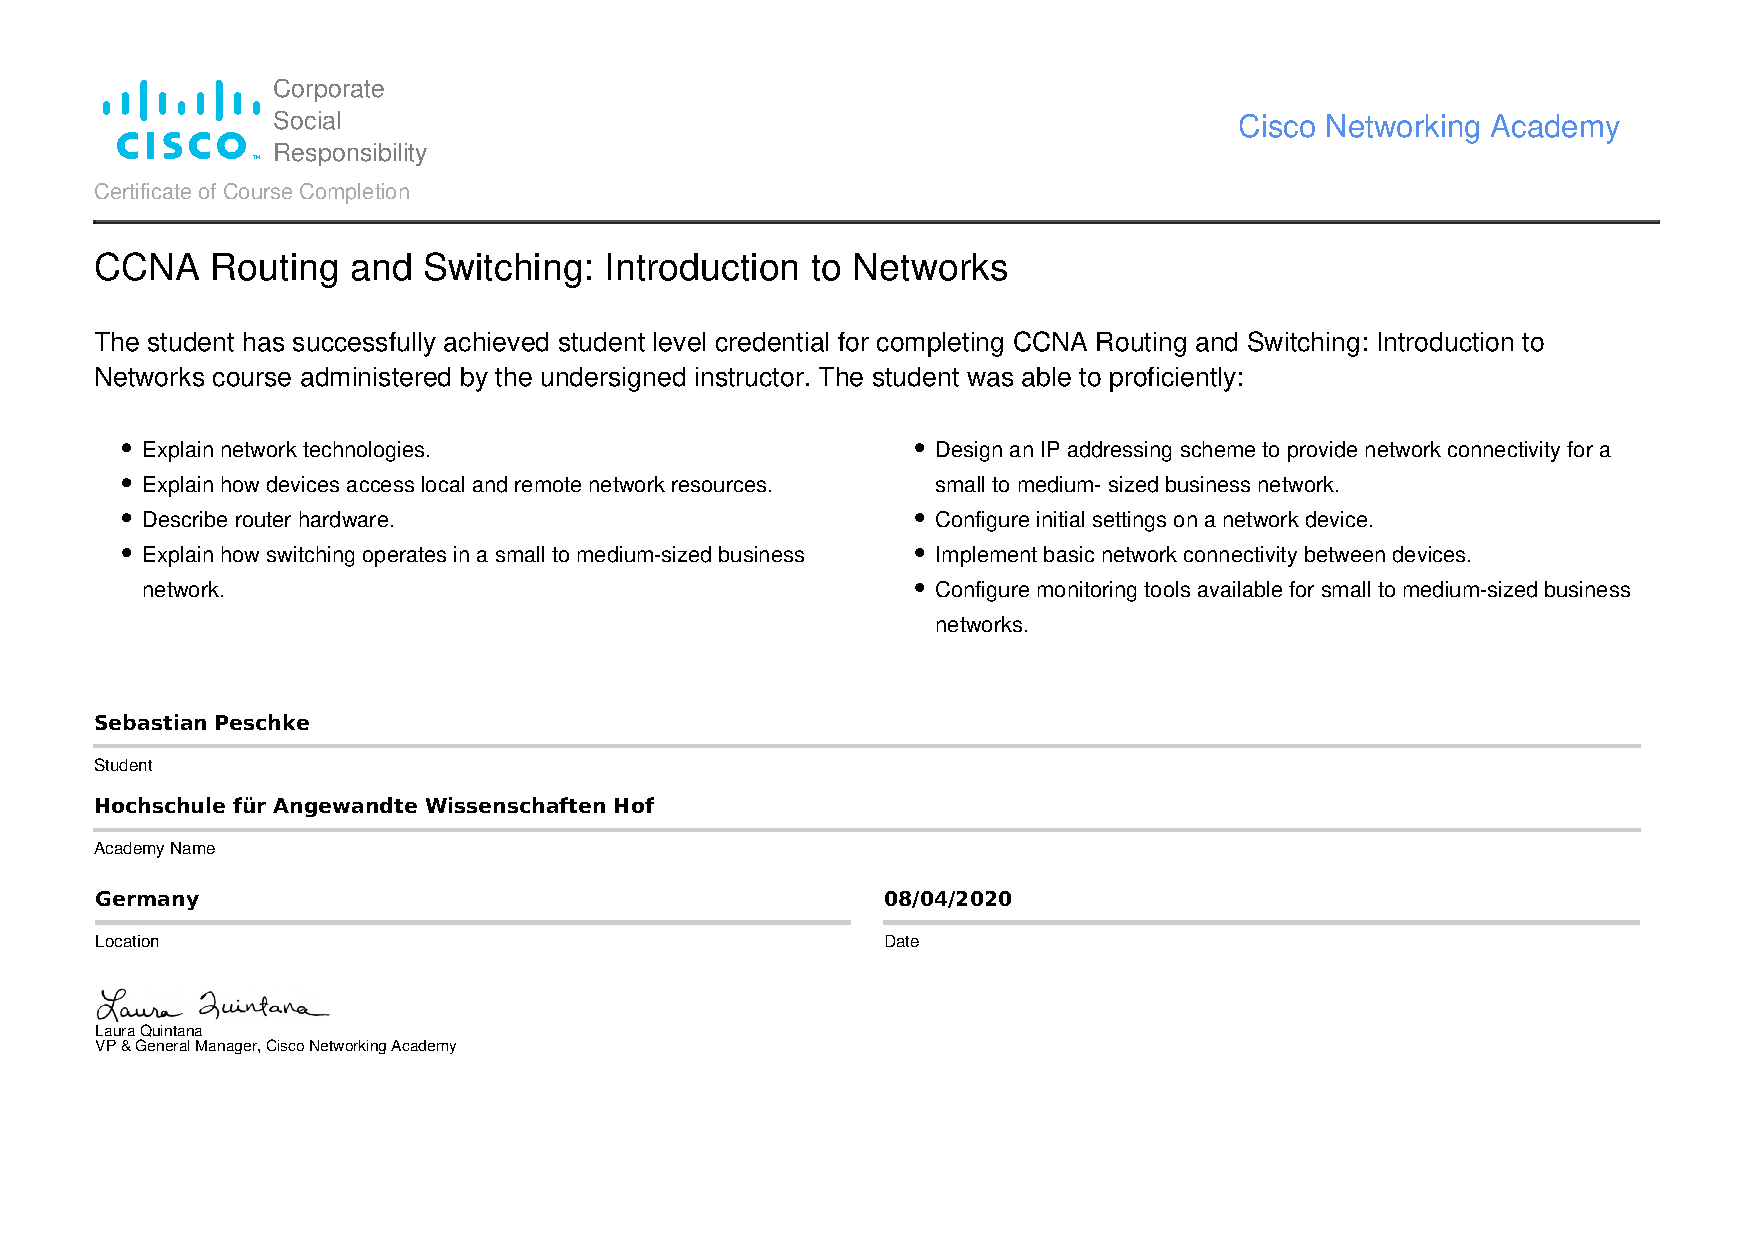
\includegraphics[scale=0.8]{./assets/SebastianPeschke-HOF_2020_I2N_HEY-certificate}
	\newpage
	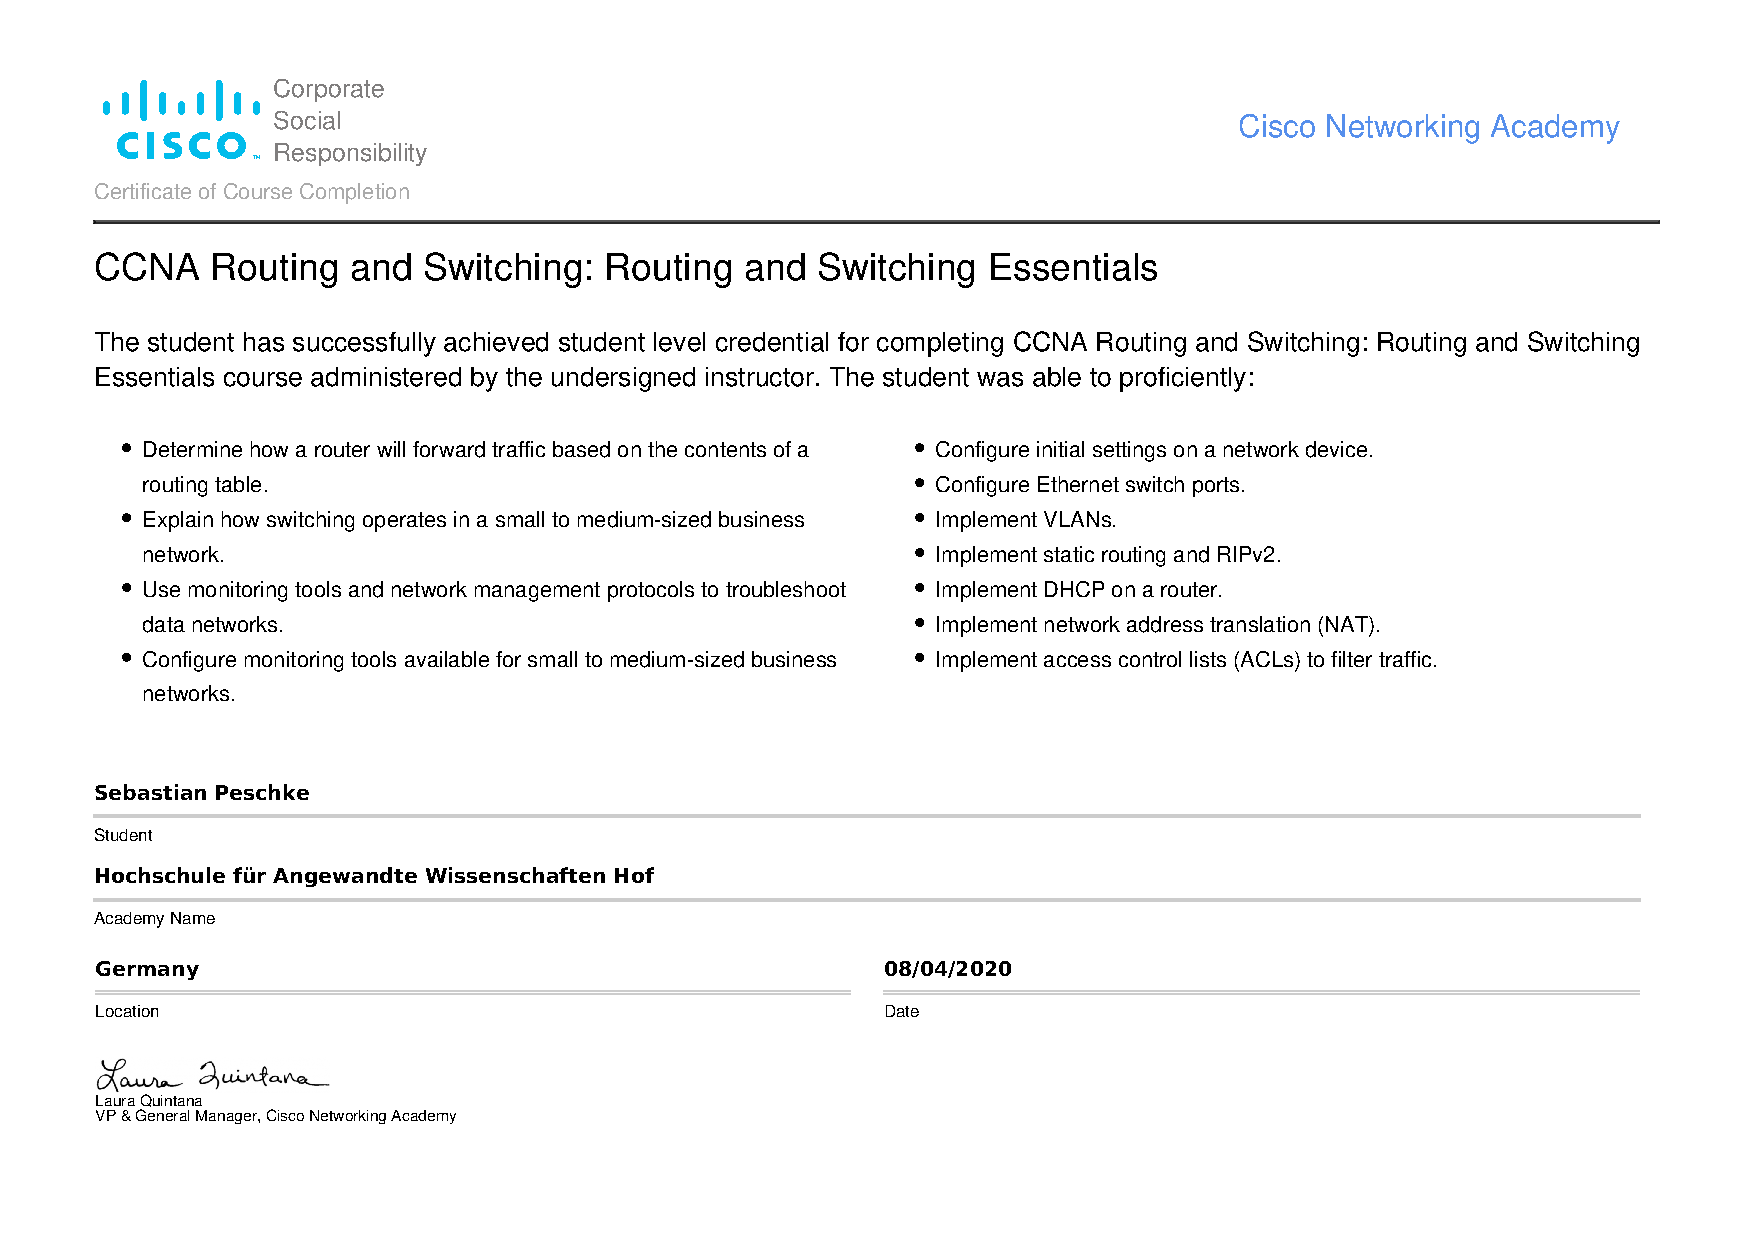
\includegraphics[scale=0.8]{./assets/SebastianPeschke-HOF_2020_RSE_HEY-certificate}
	\newpage
	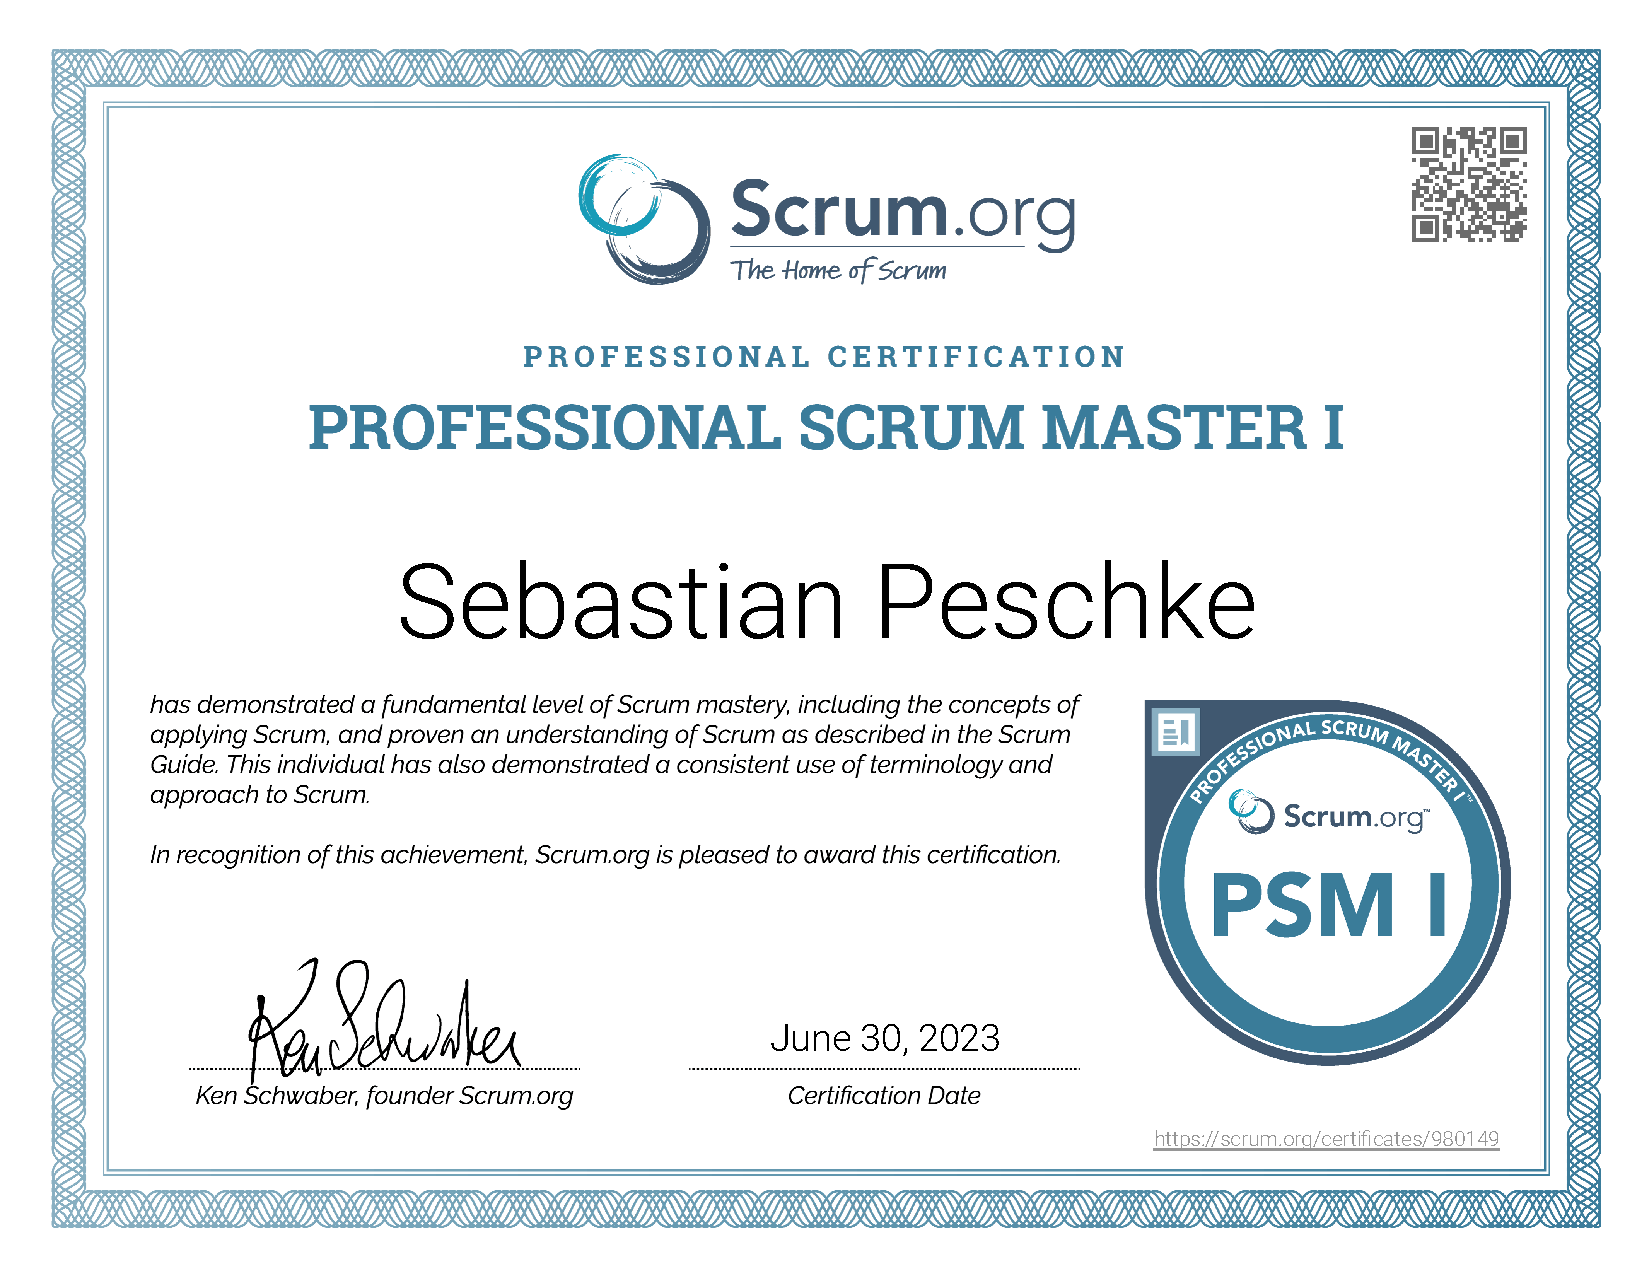
\includegraphics[scale=0.8]{./assets/Professional Scrum Master I}
\end{landscape}
\end{document}
